The intention of this report is to investigate preliminary data coming from the ITS and MFT in Run 3. The order of the discussion in this section will follow the order that we tackled things. This is done to show both the progression of our knowledge as well as to try to clarify some of the explanations in previous sections as the only way to truly understand some things is through example. 

\subsection{The Data}
The data analysed in this report was taken in October 2021, where protons were collided at a centre of mass energy of \SI{900}{\giga\electronvolt}. This is not an energy that we expect to use for physics research but it allows us to look at how the detectors are performing with more lightweight data, simply because there will be fewer particles created in the collisions and thus less data to work with. We are using runs 505548 and 505645. In this case, a run specifies a period of data taking for which all global settings remain the same. All further plots, unless specified otherwise, will include both runs.


\subsection{Initial MFT Analysis}
In the AOD data model there is a table called \texttt{MFTTracks} which contains the tracks detected in the MFT. When we began this analysis, only two reconstruction passes had been run on the data and while the MFT was switched on for the runs, the \texttt{MFTTracks} table had not been populated. We thus had to wait for pass 3 and we spent that time getting familiar with the analysis framework as described in \cref{sec:AnalysingWithO2}. With pass 3 available, the plots in \cref{fig:MFT_1D_pass3} were able to be created. The variables plotted are all available as static or dynamic columns in the AOD structure so no complicated analysis was needed to obtain them. 

\begin{figure}[h]%
    \centering
    \begin{subfigure}[t]{.49\linewidth}
        \centering
        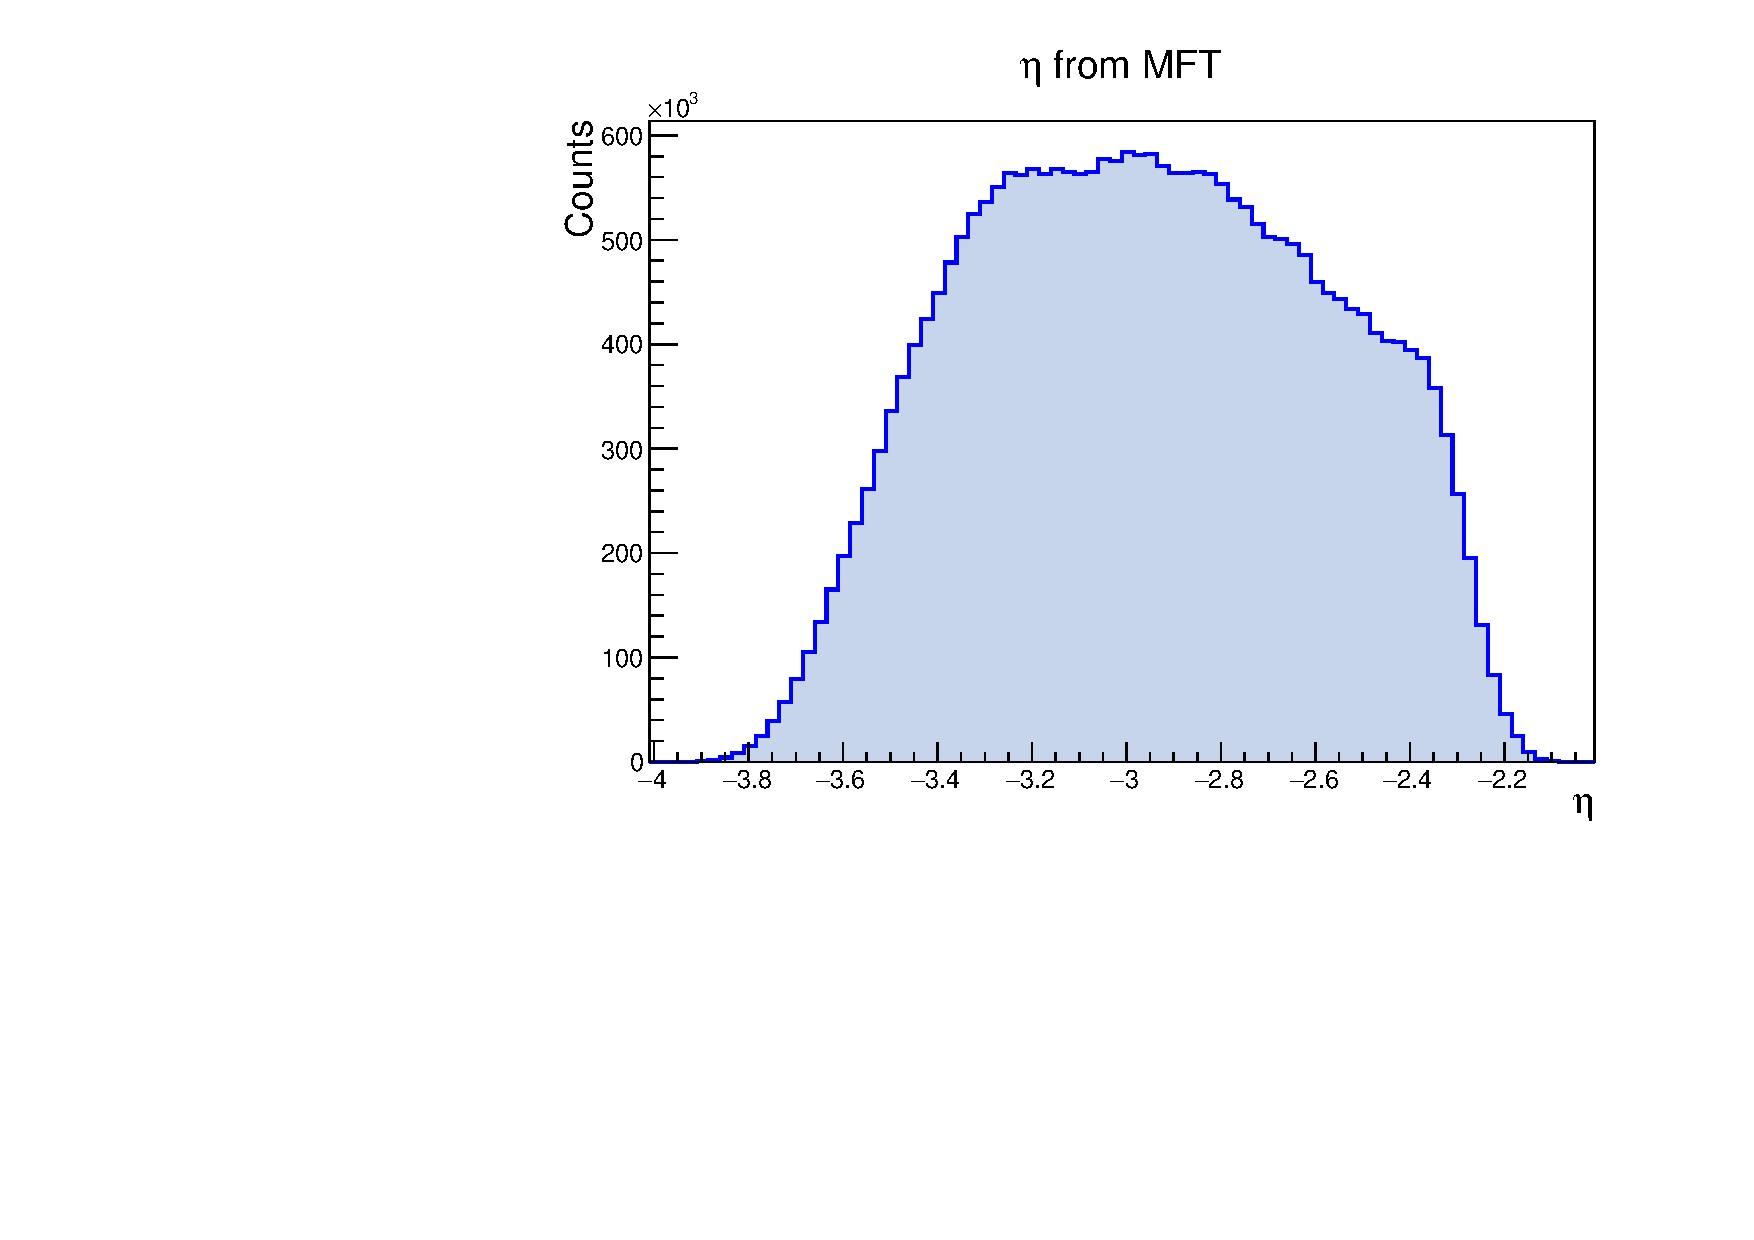
\includegraphics[width=\linewidth]{Plots/pass3_MFT/MFTeta_pass3.pdf}
        \caption{$\eta$ of tracks detected in the MFT. }
        \label{fig:MFTeta_pass3}
    \end{subfigure}
    \hfill
    \begin{subfigure}[t]{.49\linewidth}
        \centering
        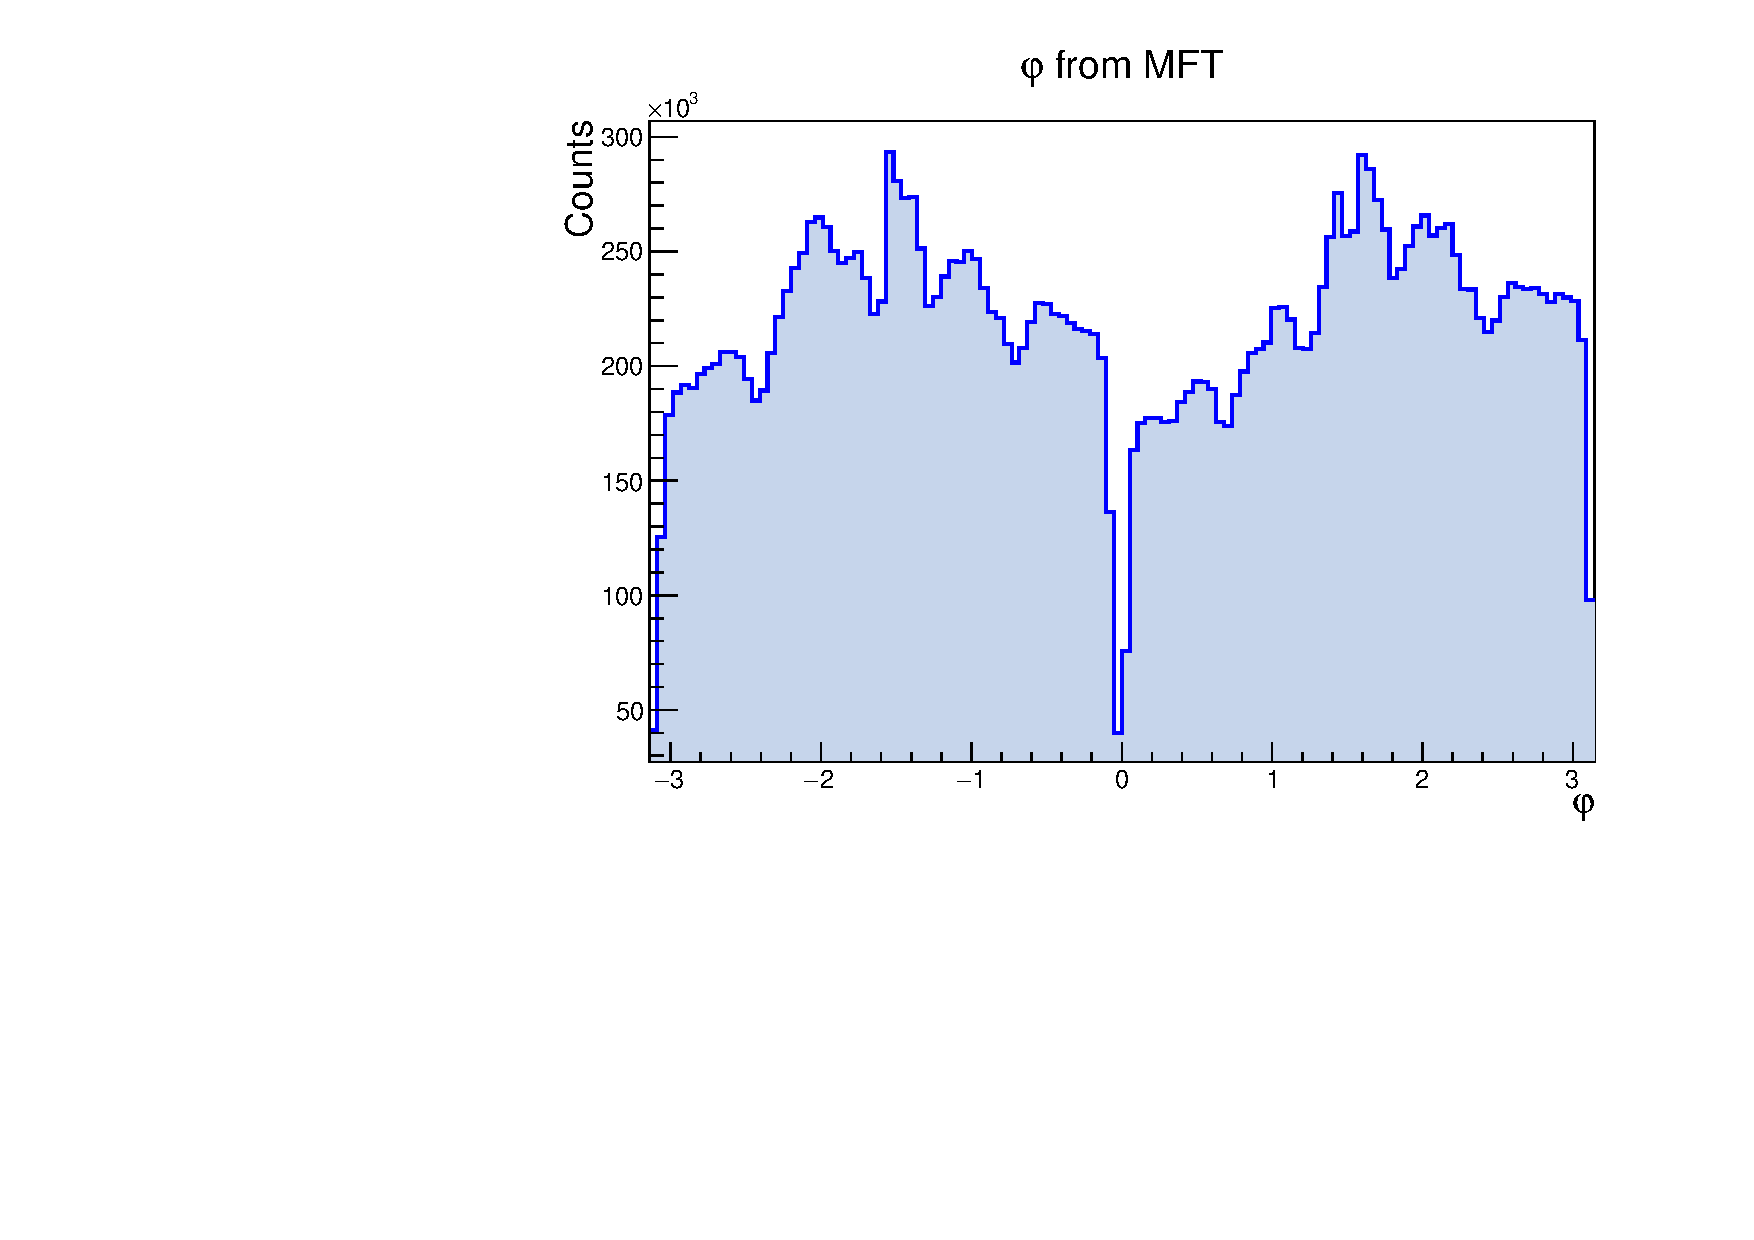
\includegraphics[width=\linewidth]{Plots/pass3_MFT/phi_pass3.pdf}
        \caption{$\varphi$ of tracks detected in the MFT. Note the range of $\varphi$.}
        \label{fig:MFTphi_pass3}
    \end{subfigure}
    \begin{subfigure}[t]{.49\linewidth}
        \centering
        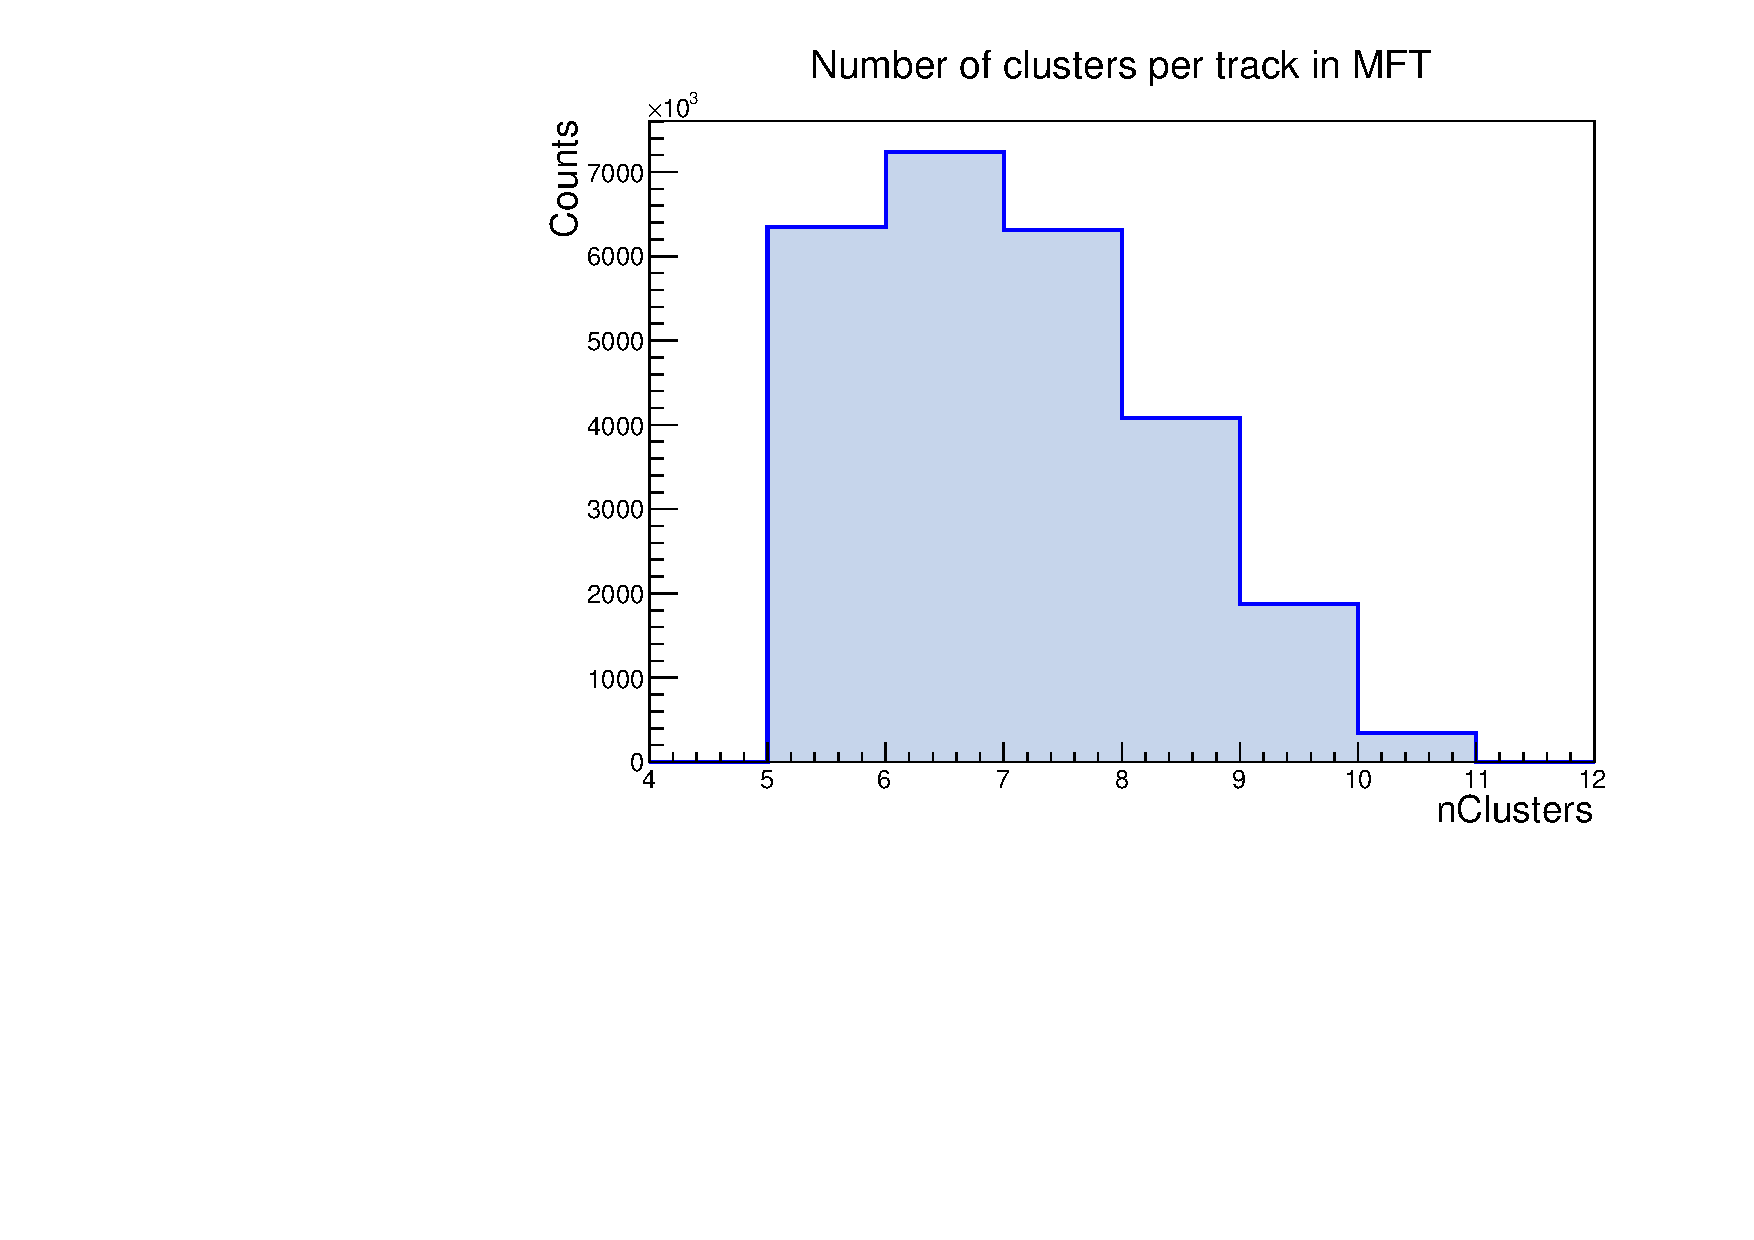
\includegraphics[width=\linewidth]{Plots/pass3_MFT/nClusters_pass3.pdf}
        \caption{Number of clusters per track detected in the MFT. Note the cut-off at 5.}
        \label{fig:MFTnClusters_pass3}
    \end{subfigure}
    \hfill
    \begin{subfigure}[t]{.49\linewidth}
        \centering
        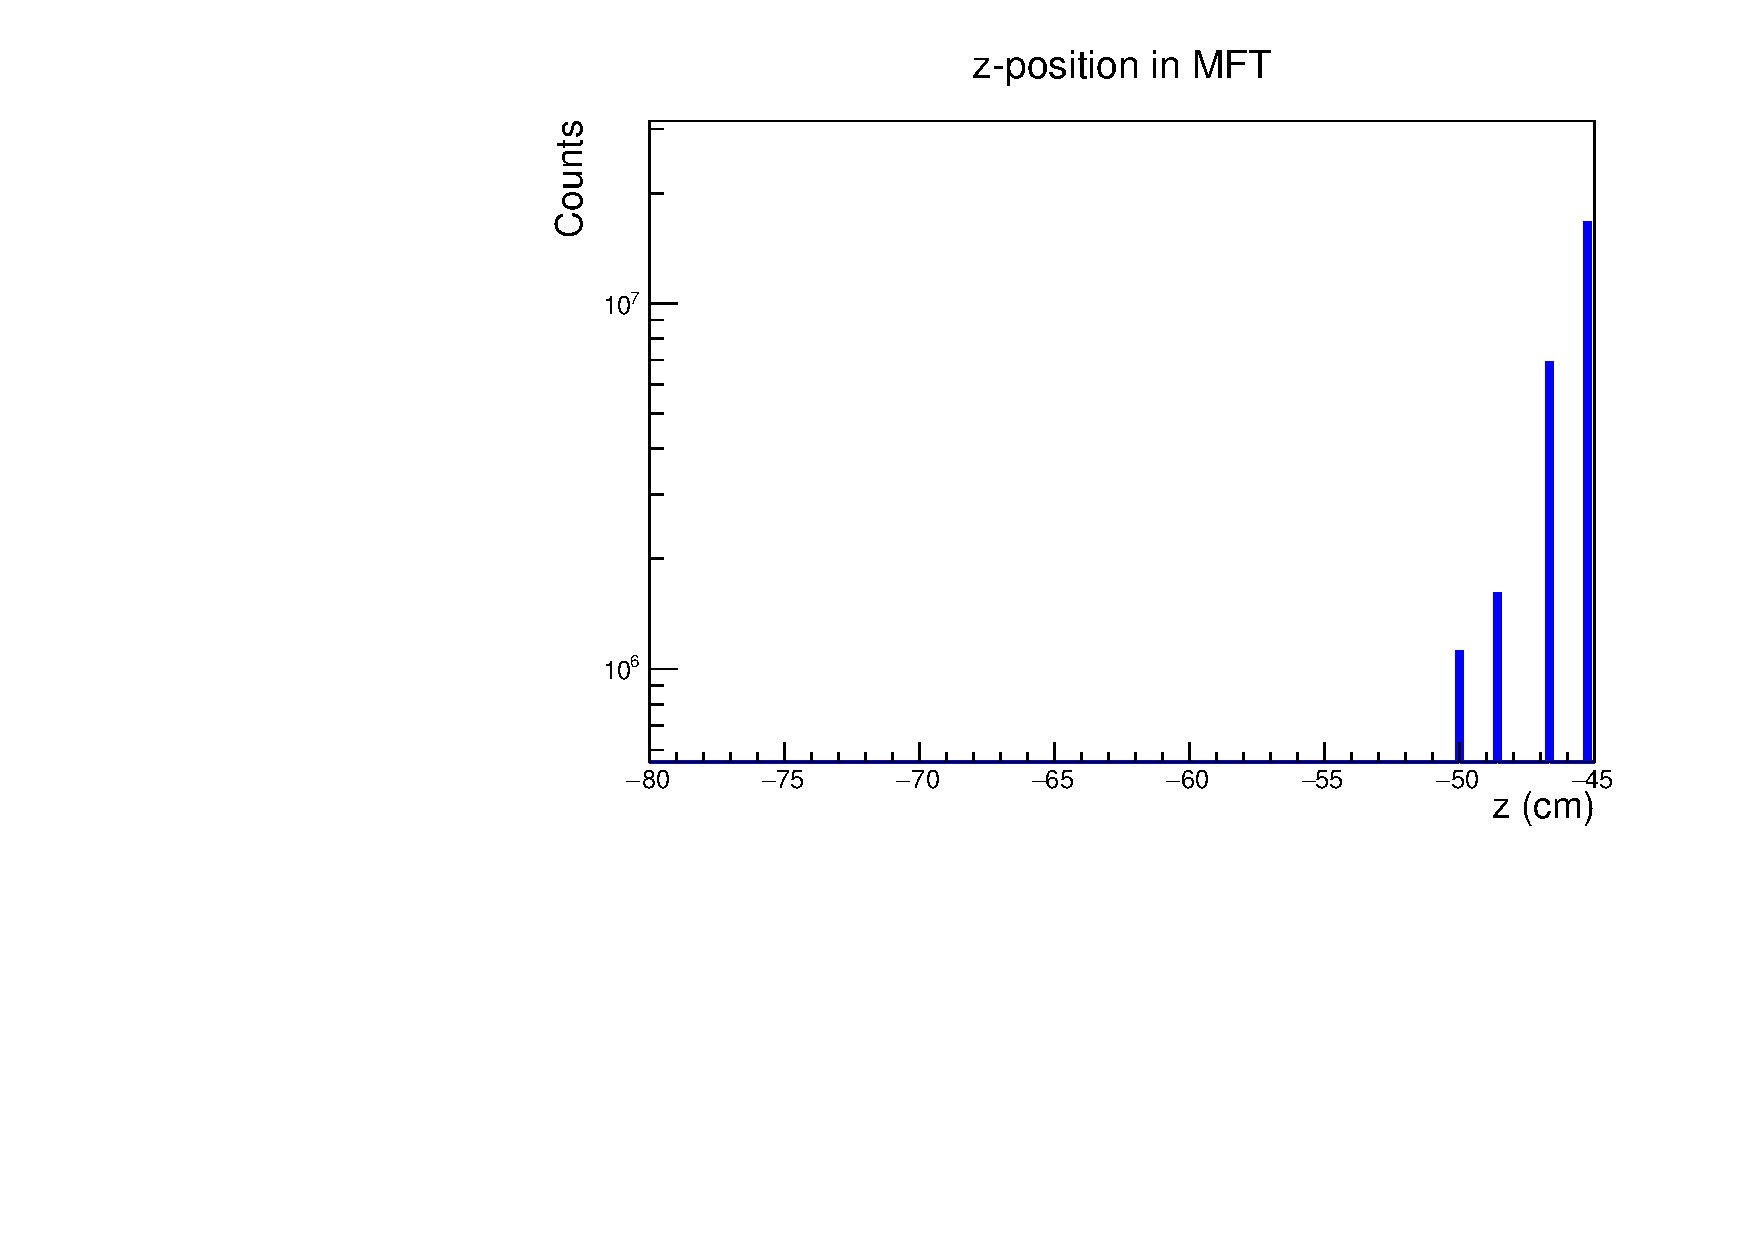
\includegraphics[width=\linewidth]{Plots/pass3_MFT/Z_MFT_pass3.pdf}
        \caption{$z$-position of first hit in the MFT. Note how the $z$ range covers the whole MFT but only the first 4 detector planes have hits.}
        \label{fig:Z_MFT_pass3}
    \end{subfigure}
\caption{1-D histograms for some kinematic variables as well as the number of clusters per track in the MFT. Data from reconstruction pass 3. }
\label{fig:MFT_1D_pass3}
\end{figure}

Starting with $\eta$, we see the distribution is lopsided to the lower $\eta$ values but it's not as smooth in the middle as we might expect from a detector with continuous sensitive material in those regions. We will investigate this more in \cref{sec:comapring}. The $\varphi$ plot shows the structure of the MFT quite well. The valley at the centre shows the gap between the top and bottom half-disks and the spikes come from the fact that the sensitive area of each disk is not perfectly circular, so there will be directions that can detect more tracks than others. 

The number of clusters per track is interesting. As was mentioned in \cref{sec:MFT_Theory}, the MFT requires a track to be detected in 4 out of the 5 disks in order to be considered a track. The translation of that statement into number of clusters per track is a bit unclear but we might expect that the minimum number of clusters per track should be 4 as each disk has 2 planes but the track only needs to have a cluster in one of them to count towards the 4 out of 5. However, what we see in \cref{fig:MFTnClusters_pass3} is a minimum of 5 clusters per track. This might be down to a choice made in the reconstruction process to instead require that all 5 disks detect the track before it is accepted. It could also be due to a physical limitation where it's simply not possible for 4 disks to detect a track and not see clusters in 5 disks. At the point of writing, we have not been able to determine the reason for this as the details of reconstruction are near impossible to find.

Interpreting \cref{fig:Z_MFT_pass3} was its own adventure. The documentation for the AOD data model is unclear what gets calculated for the $z$ column in the \texttt{MFTTracks} table, but we believe that it represents the $z$-position of the first hit (or cluster) of a given track in the MFT. We see that after the fourth plane, i.e. the second disk, there is no data. This supports the fact that 4 out of 5 disks are required to accept a track as having a first hit in the third disk will obviously never result in a track hitting 4 disks. This information seems to be contradicting the information from \cref{fig:MFTnClusters_pass3} but we regrettably have no resolution to the situation.

\bigskip

Out of interest, we can look at the $x$ and $y$ positions of the hits in the first 4 layers that we saw in \cref{fig:Z_MFT_pass3}. This is shown in \cref{fig:MFT_x_y_pass3} and the structure of the ladders of pixel detectors can clearly be seen. As with the $z$ plot, there is no further data for the other layers in the MFT. It would be useful to be able to see the positions of all of the hits for a track, but we are restricted to what is added to the AOD and at this point, this is all we have to work with. 

The blank regions in the $x$-$y$ plots are likely areas where the data has been masked. This is most likely to be because the detector had high noise levels in those areas, which would blow out the rest of the data. Looking at the first two plots, we can see how the front and back planes of the first disk are offset from each other, as we saw in \cref{fig:MFT_Disk4_mapping}. We also see an increased number of hits closer to the centre of the disks. This can be explained by the fact that, assuming particles are emitted isotropically from the interaction point, there will be a drop-off in density of particles as the distance from the interaction point increases and since the disks are flat, the larger the radius on the disk, the further from the interaction point. Thus the density of hits should decrease as the disk radius increases. 

\begin{figure}[H]%
    \centering
    \begin{subfigure}[t]{.45\linewidth}
        \centering
        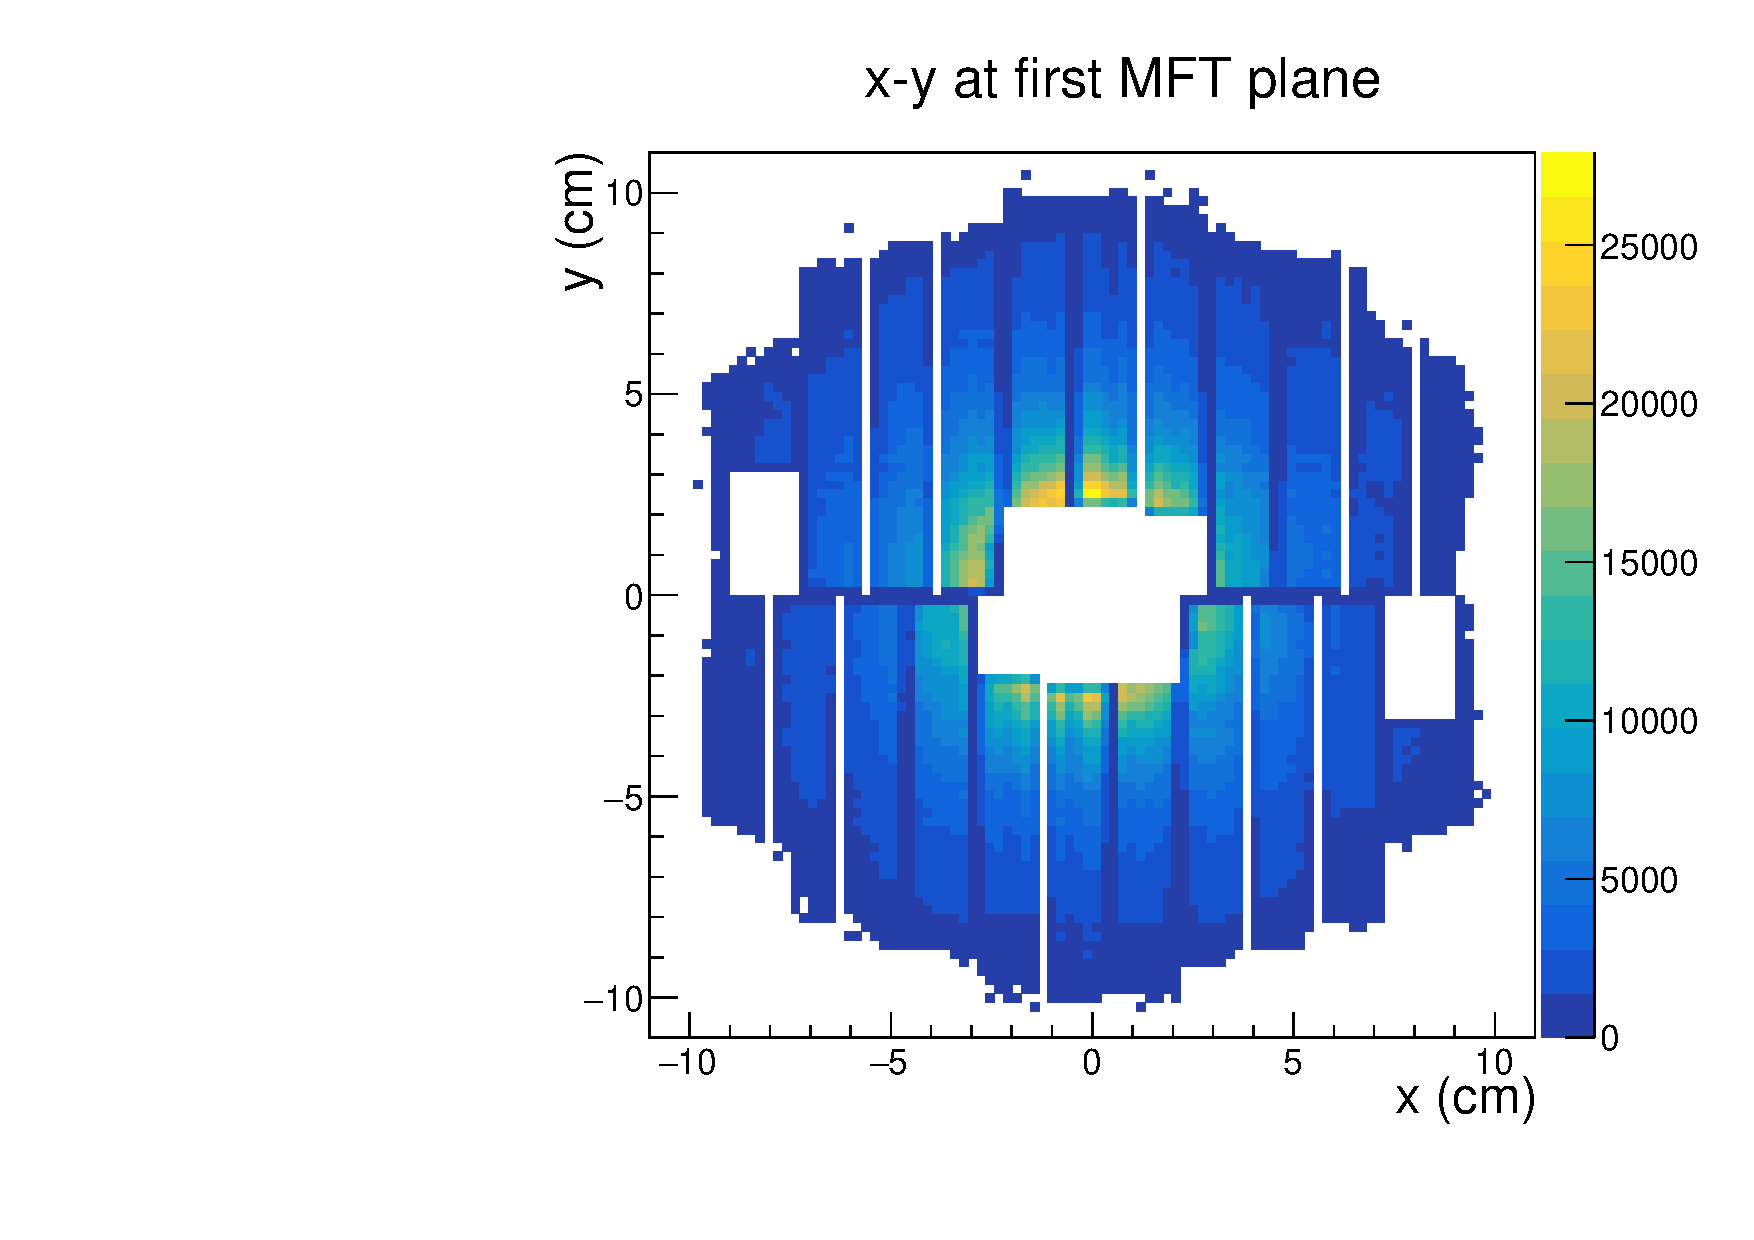
\includegraphics[width=\linewidth]{Plots/pass3_MFT/x_y_1_pass3.pdf}
        \caption{}
        \label{fig:x_y_1_pass3}
    \end{subfigure}
    \hfill
    \begin{subfigure}[t]{.45\linewidth}
        \centering
        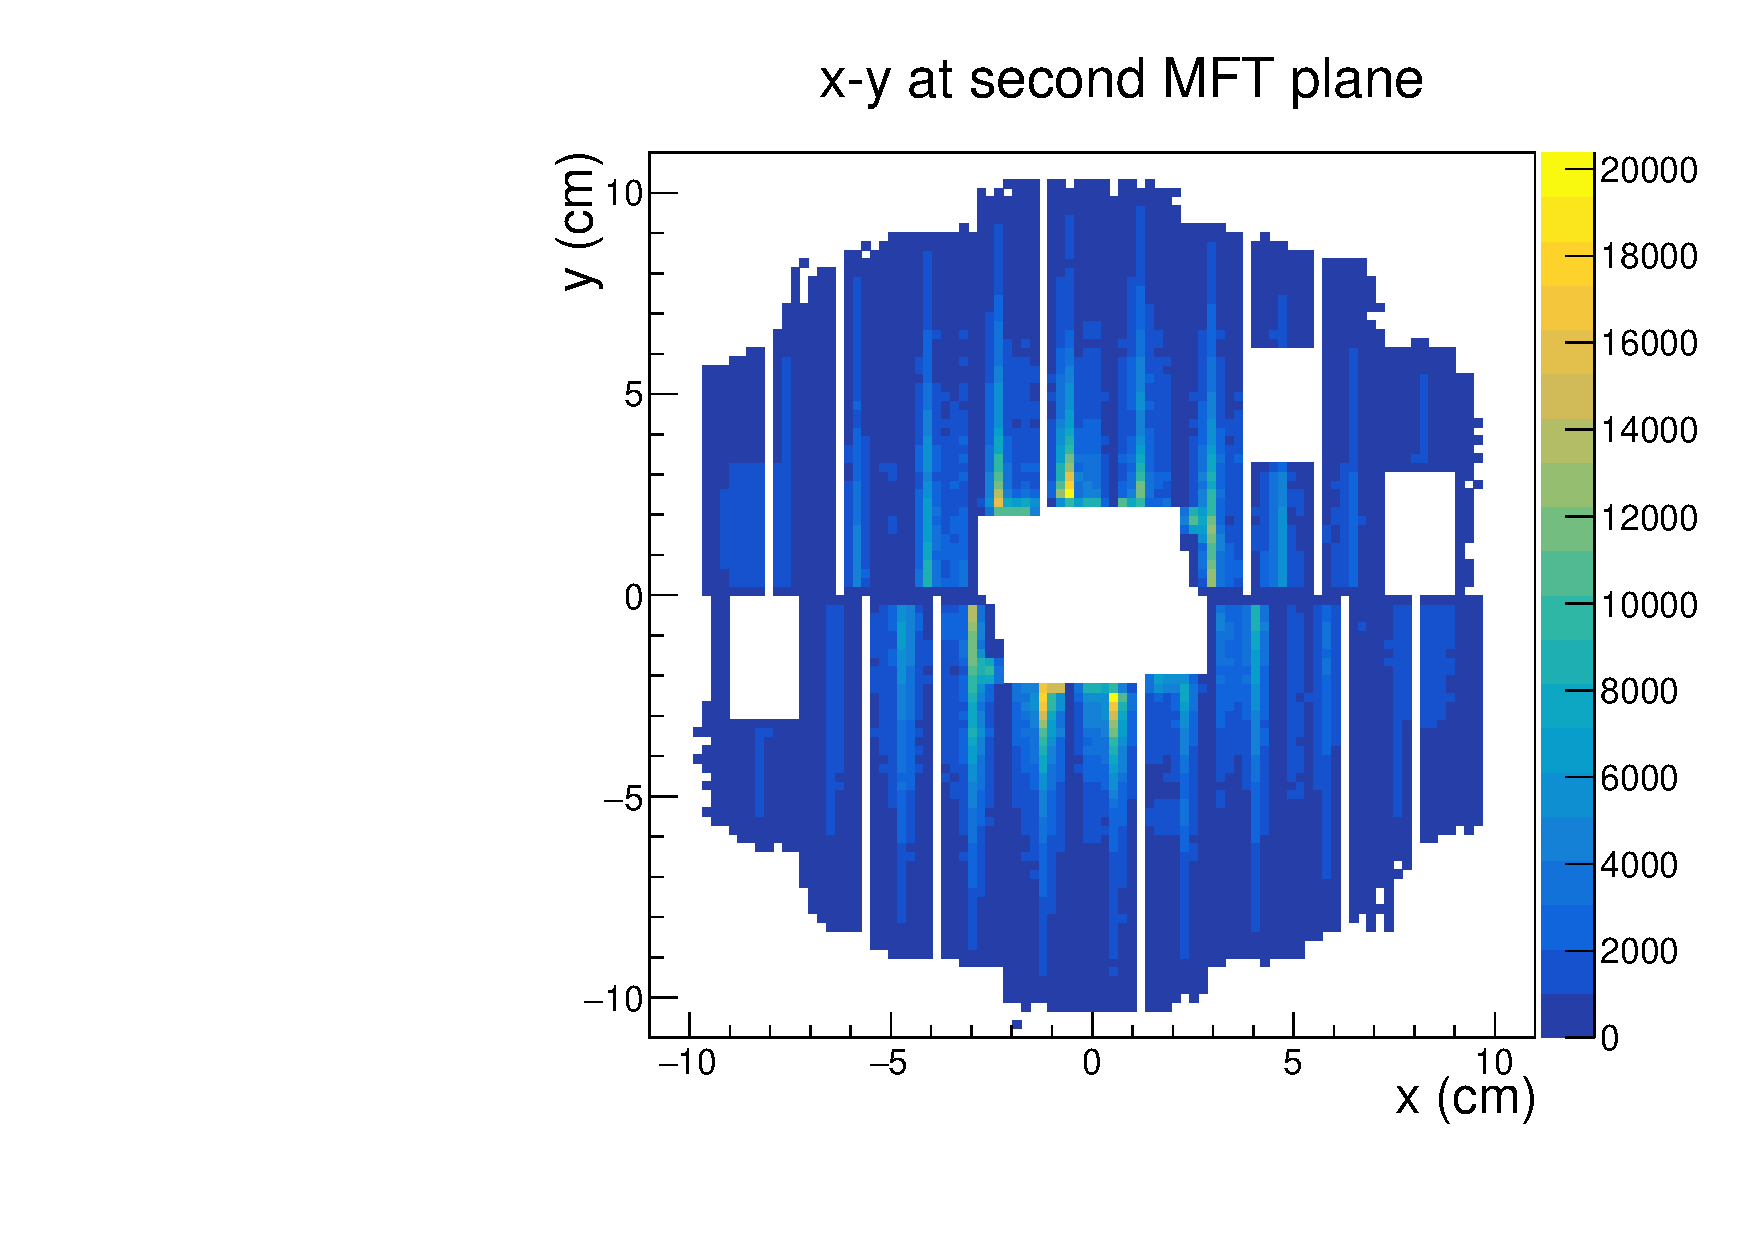
\includegraphics[width=\linewidth]{Plots/pass3_MFT/x_y_2_pass3.pdf}
        \caption{}
        \label{fig:x_y_2_pass3}
    \end{subfigure}
    \begin{subfigure}[t]{.45\linewidth}
        \centering
        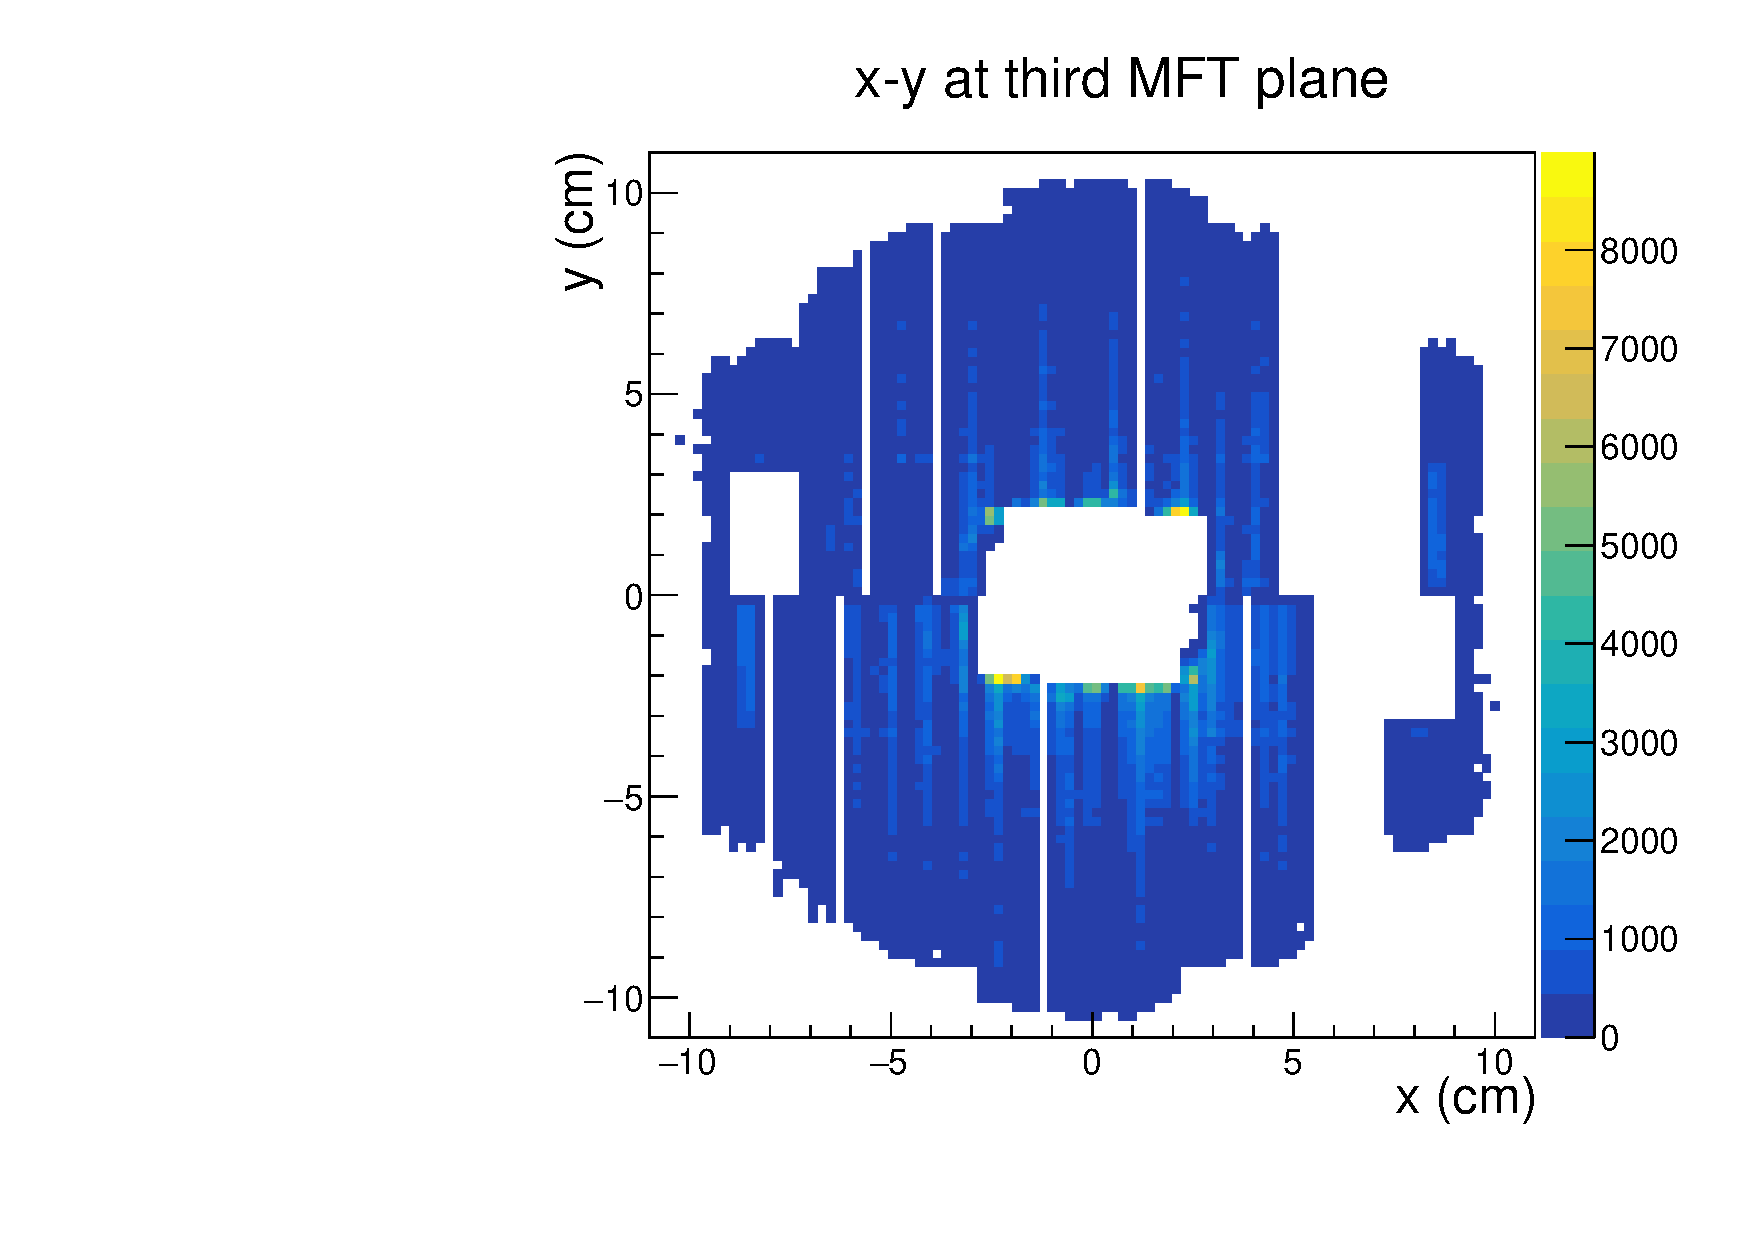
\includegraphics[width=\linewidth]{Plots/pass3_MFT/x_y_3_pass3.pdf}
        \caption{}
        \label{fig:x_y_3_pass3}
    \end{subfigure}
    \hfill
    \begin{subfigure}[t]{.45\linewidth}
        \centering
        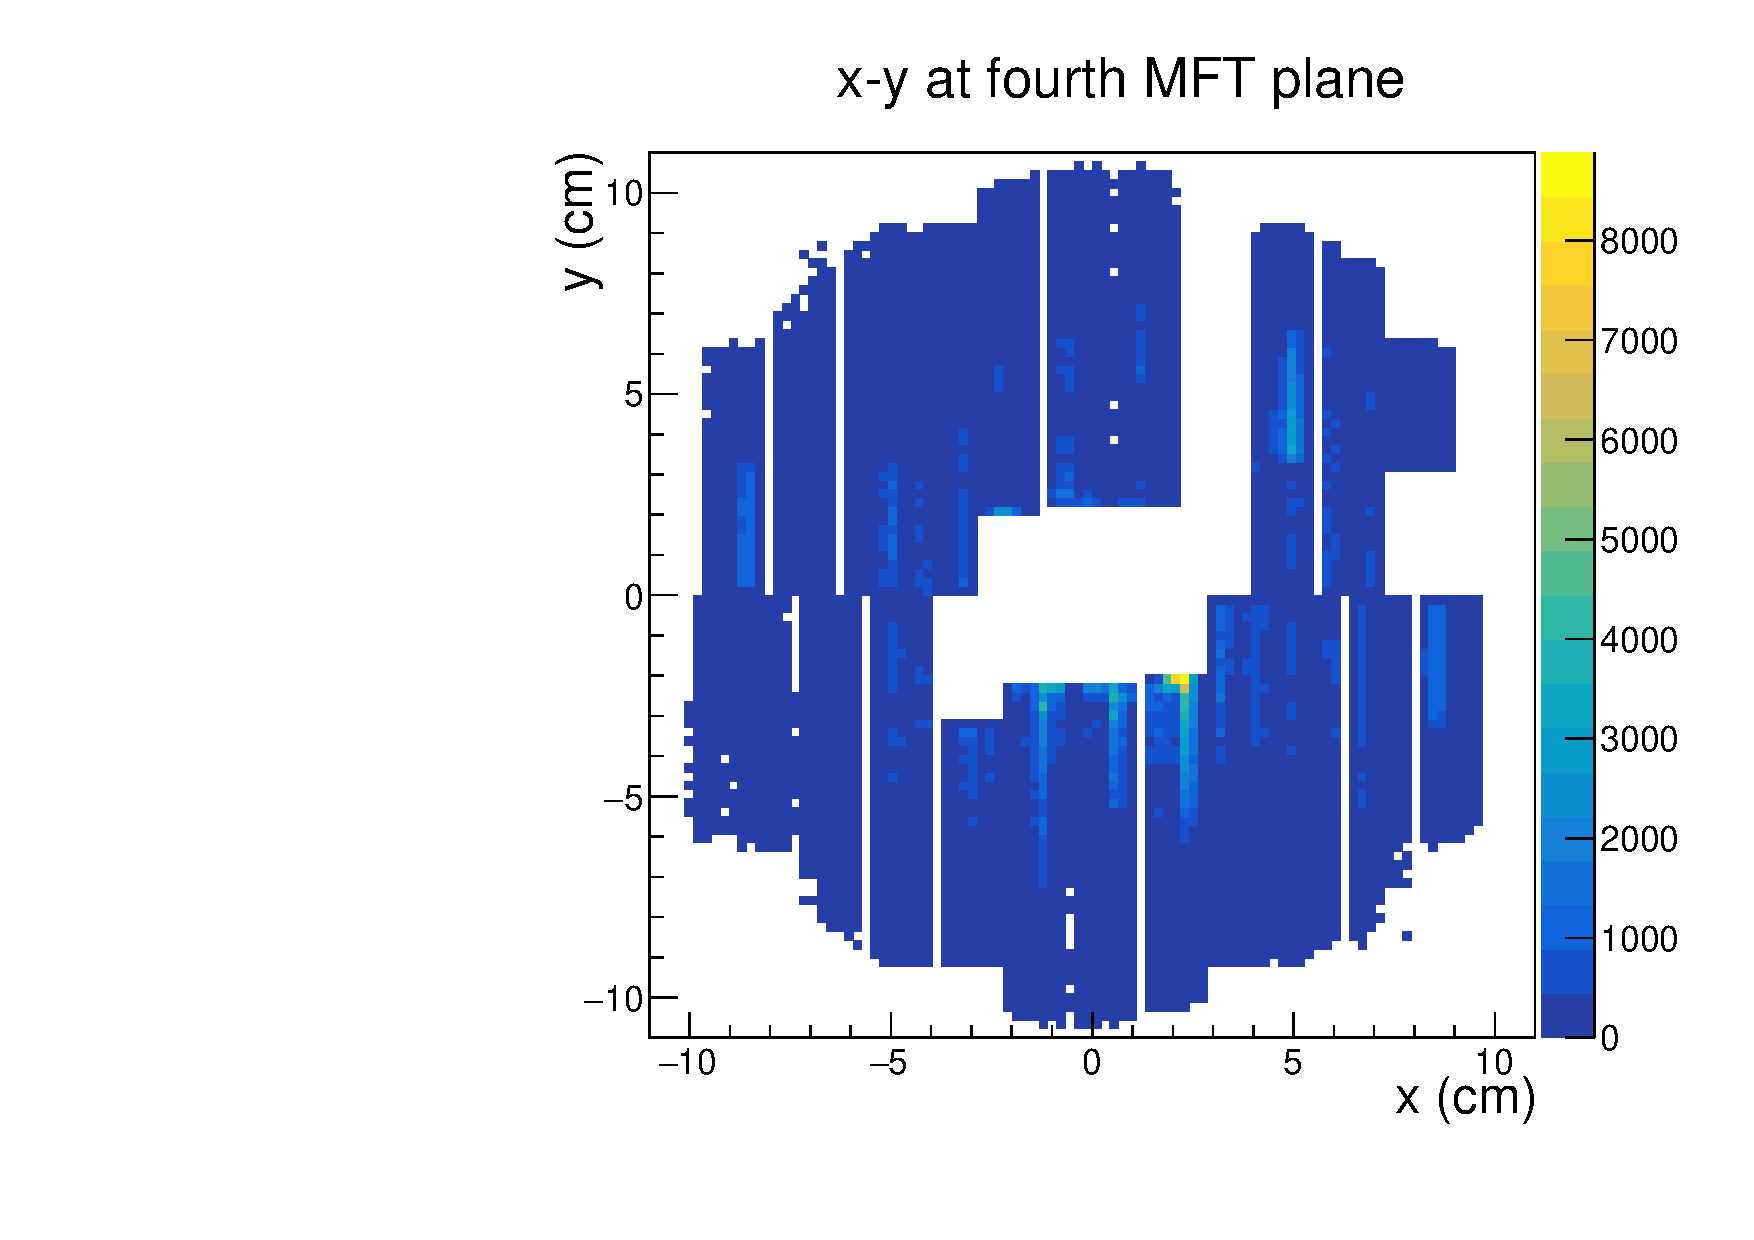
\includegraphics[width=\linewidth]{Plots/pass3_MFT/x_y_4_pass3.pdf}
        \caption{}
        \label{fig:x_y_4_pass3}
    \end{subfigure}
\caption{$x$ and $y$ positions of hits in the first 4 layers of the MFT. This is related to \cref{fig:Z_MFT_pass3} as these are the first hits for a given track, so looking at the later layers yields no data. The sections with no data have likely been masked out to remove regions of abnormally high noise. Important to note how at the centre of the disk we see a higher hit density than further out.}
\label{fig:MFT_x_y_pass3}
\end{figure}

The last interesting plot from reconstruction pass 3 is a 2-D histogram of $\eta$ and $\varphi$. \Cref{fig:eta_phi_pass3} shows this and we can immediately see the resemblance to the layout in \cref{fig:MFT_Disk4_mapping}. As with \cref{fig:MFTphi_pass3}, we can see the gap in between the half-disks. 

\begin{figure}[h]
    \begin{center}
        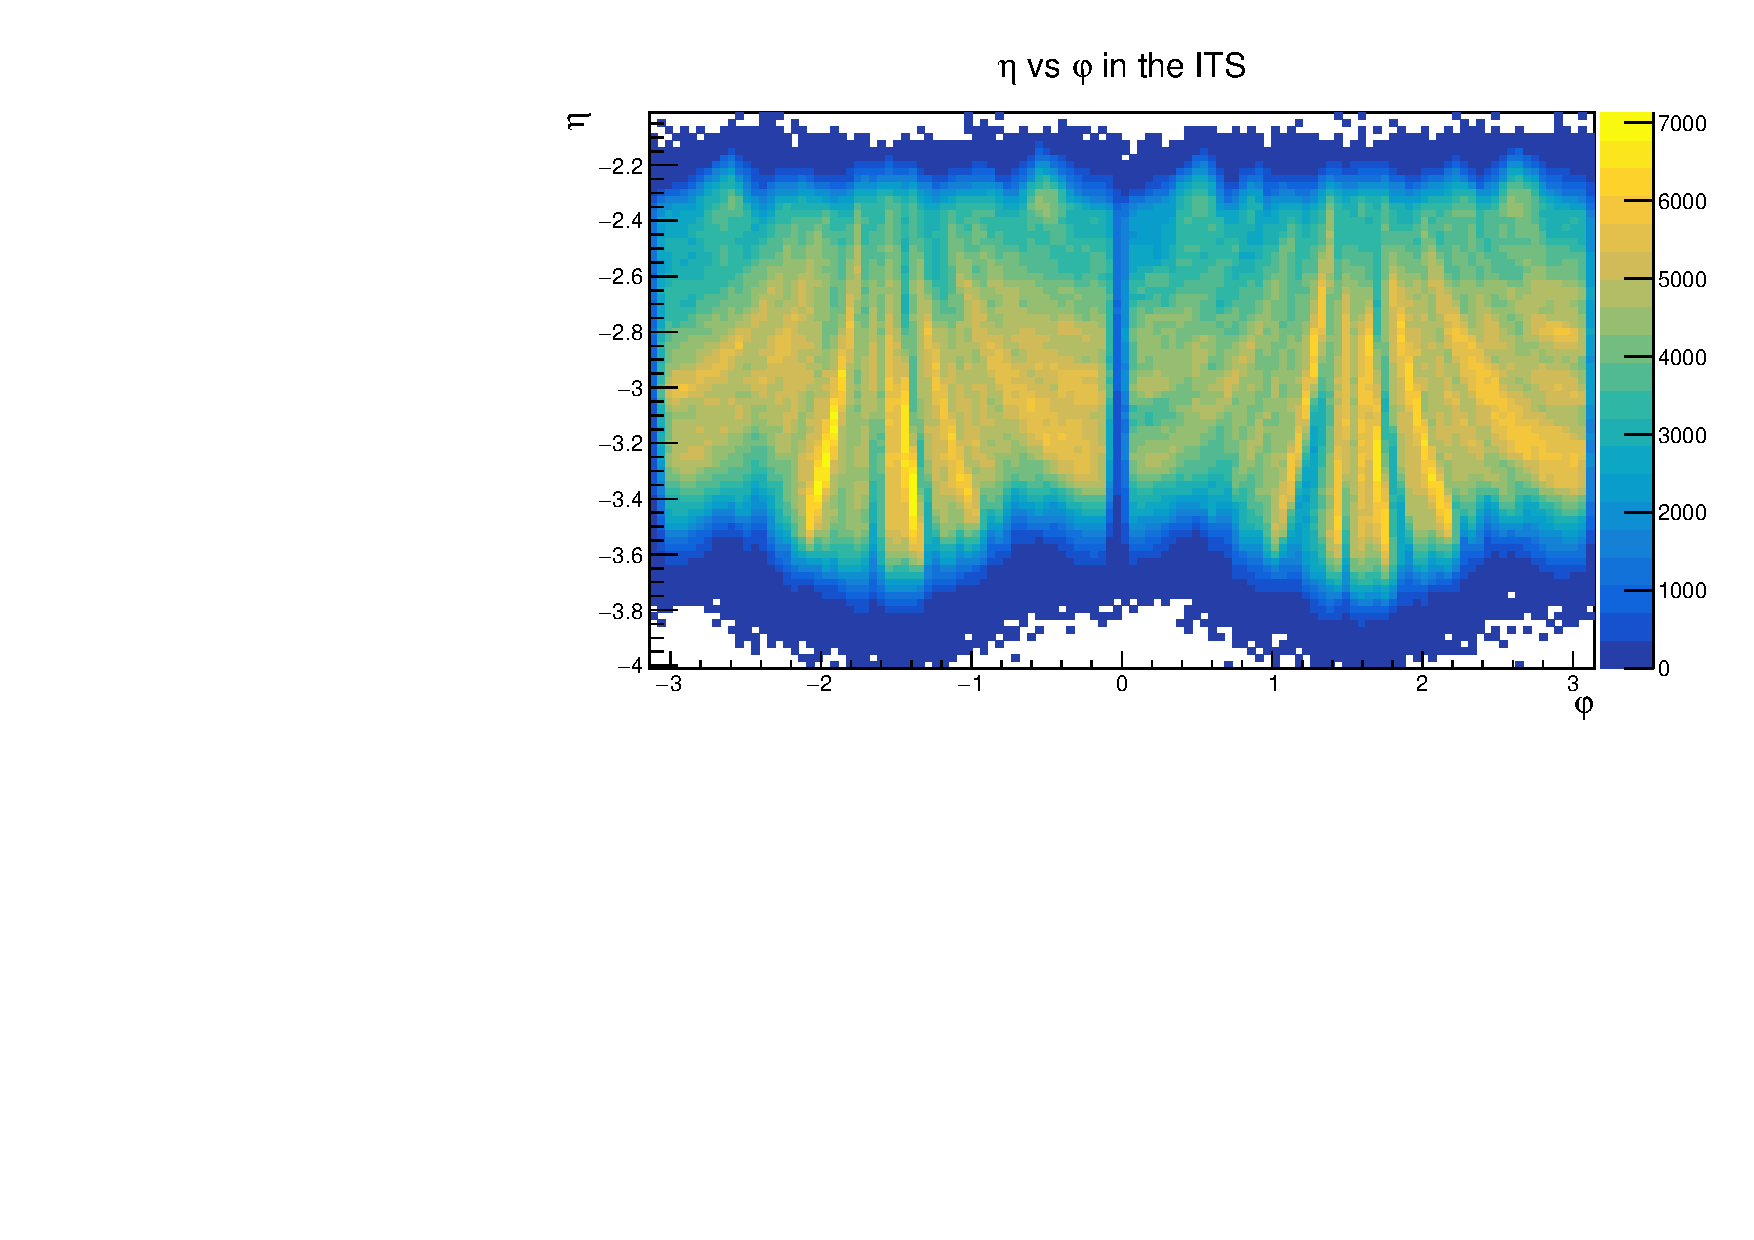
\includegraphics[width=.8\textwidth]{Plots/pass3_MFT/eta_phi_pass3.pdf}
        \caption{Histogram of $\eta$ and $\varphi$ for tracks in the MFT. The half-disk structure can clearly be seen when comparing to \cref{fig:MFT_Disk4_mapping}. }
        \label{fig:eta_phi_pass3}
    \end{center}
\end{figure}

\subsection{Comparing pass 3 to pass 4}\label{sec:Comapring}
In \cref{fig:MFTeta_pass3} we can see that the distribution looks slightly jagged from about -2.4 to -3.4, especially when compared to the section between -3.4 and -4. There isn't any reason to expect a non-smooth distribution there, and that viewpoint is supported by looking at the distribution after reconstruction pass 4. Some issues were identified with pass 3 so pass 4 was performed and we have plotted the two $\eta$ distributions in \cref{fig:pass3_pass4_eta} for comparison.

\begin{figure}[H]
    \begin{center}
        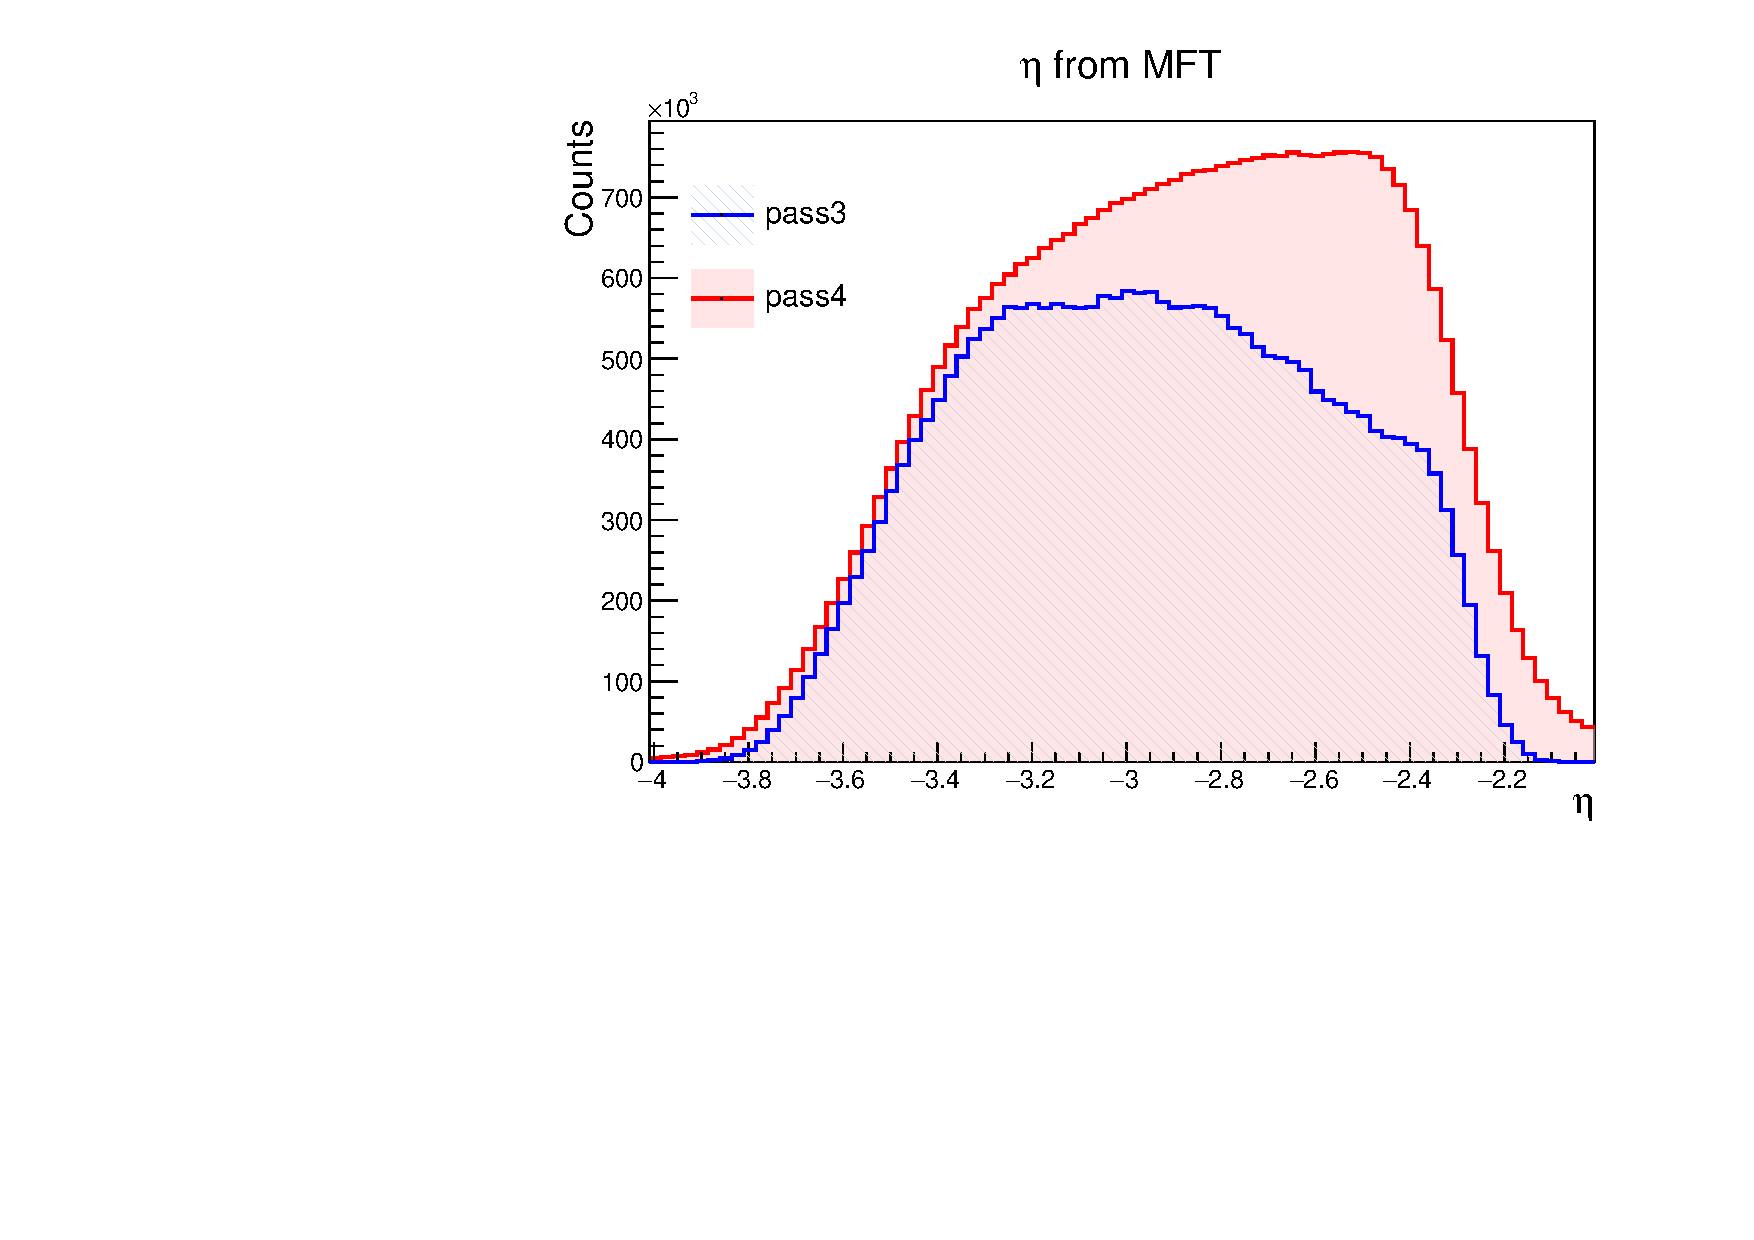
\includegraphics[width=.8\textwidth]{Plots/pass3_pass4.pdf}
        \caption{Comparison of the distribution of $\eta$ per track for reconstruction pass 3 and pass 4. We notice that there is an overall increase in number of tracks, as well as a large number of tracks added in one region, leading to an overall more smooth distribution in pass 4. Note also how there seems to be a higher density of tracks in the smaller $\eta$ range before it drops off outside the range of the MFT.}
        \label{fig:pass3_pass4_eta}
    \end{center}
\end{figure}

What we can see in \cref{fig:pass3_pass4_eta} is that pass 3 seems to have missed a large chunk of tracks in one specific region of $\eta$ compared to pass 4. The reason for this is unclear as the details of reconstruction are very hard to find but it could be due to considering MCH tracks being connected to MFT tracks. These new tracks, and thus new $\eta$ distribution, seem to contradict the conclusion drawn from the $x$-$y$ plots in \cref{fig:MFT_x_y_pass3}, where we saw a higher density of 



\begin{figure}[h]
    \begin{center}
        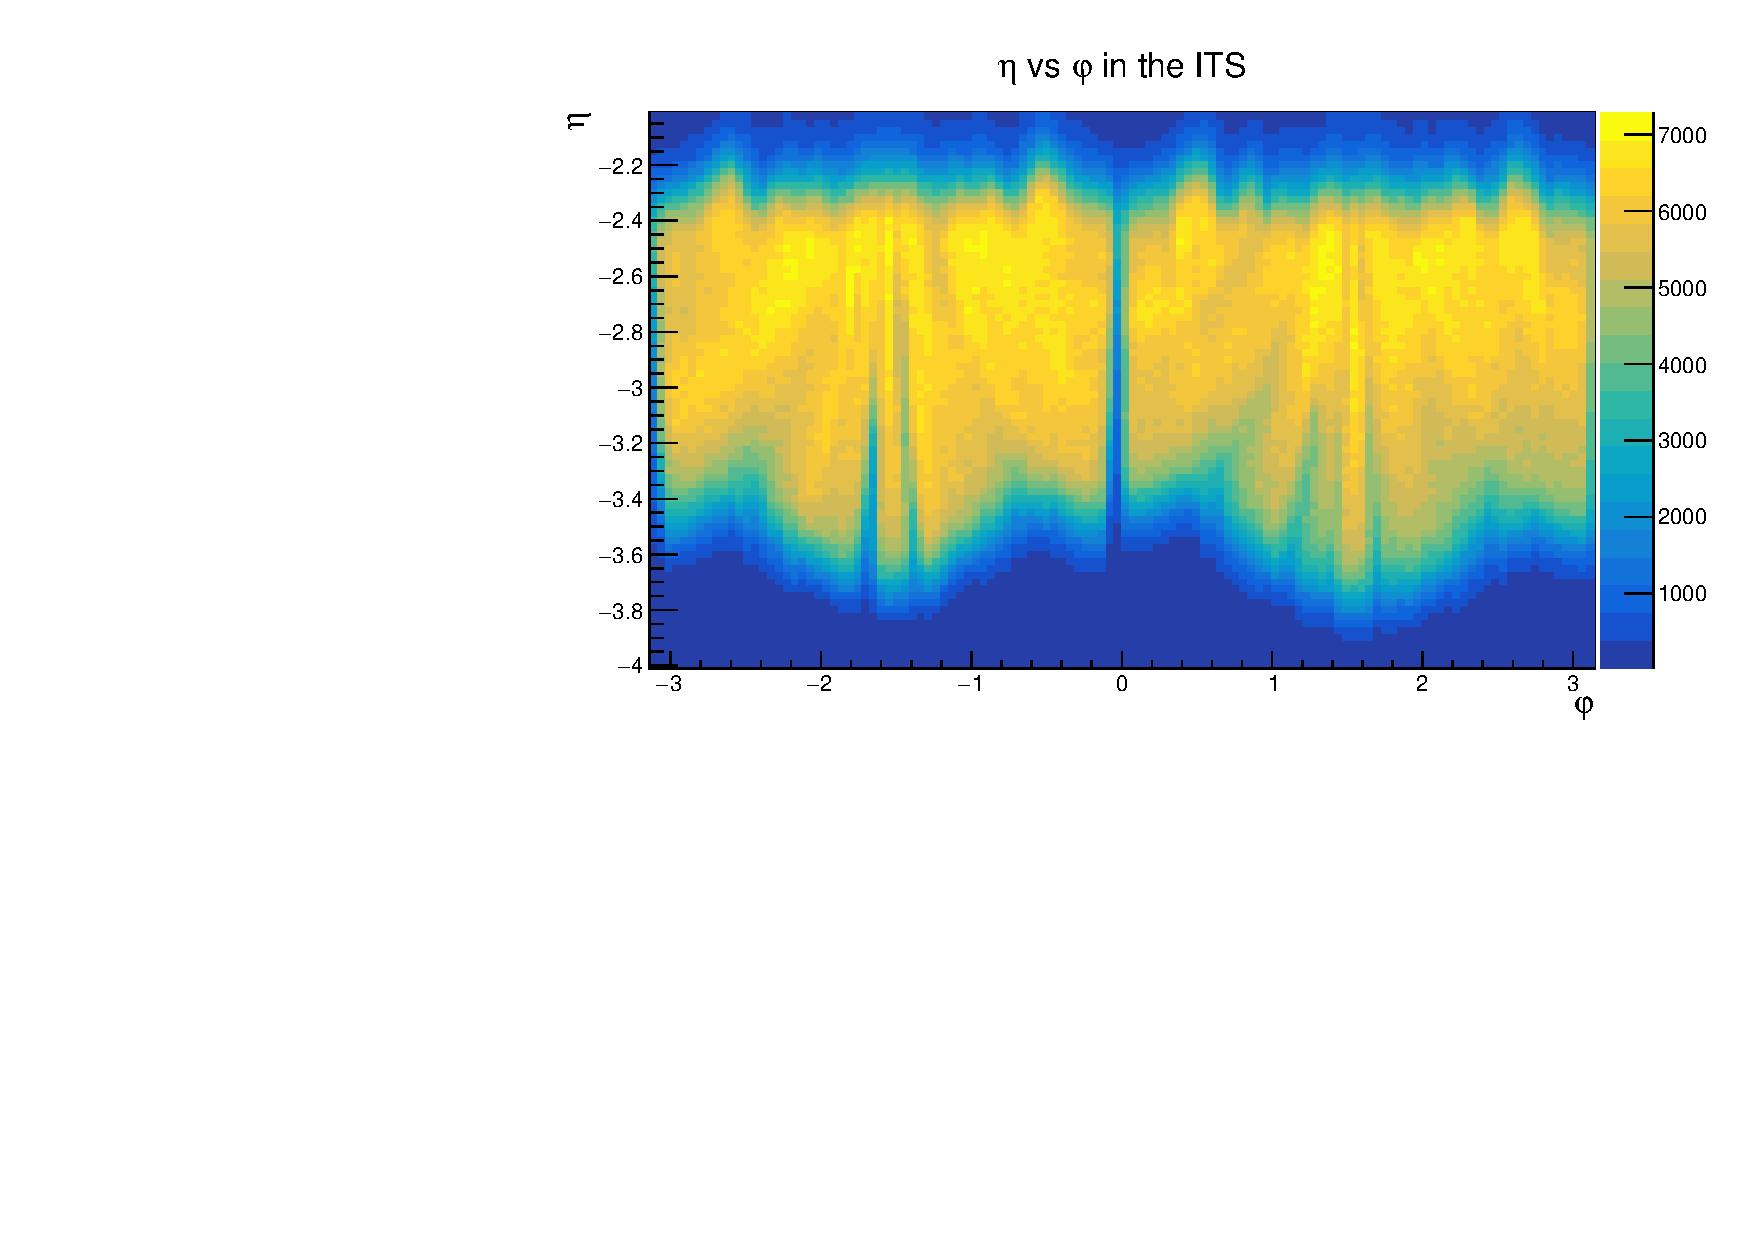
\includegraphics[width=.8\textwidth]{Plots/pass4_MFT/eta_phi_pass4.pdf}
        \caption{caption}
        \label{fig:eta_phi_pass4}
    \end{center}
\end{figure}





\subsection{Initial ITS Analysis}


\subsection{Using pass4 for hasITS}